\subsection{Kinematik}
\label{sec:sekv-kinematik}

En skitse af situationen efter det sekundære henfald ses på \cref{fig:secundary}.
\begin{figure}[h]
  \centering
  \includegraphics[width=0.6\columnwidth]{Sekventiel-kinematik}
  \caption{Skitse af situationen af det sekundære henfald. Vektorerne angiver hastighederne. $\phi$ er
    vinklen mellem hastigheden af beryllium og de sekundære $\alpha$-partikler i CM for beryllium. $\phi_{2i}$ er
    de tilsvarende vinkler i LAB-systemet.}
  \label{fig:secundary}
\end{figure}

Både i laboratorie- (LAB) og massemidtpunktsystemet (CM) følger af energi og impulsbevarelse,
at energien af de to primære henfaldsprodukter må være
\begin{equation}
  \label{eq:Ealpha0}
  E_{\alpha_{0}} = \frac{2}{3} Q_{1} \qquad E_{\ce{Be}} = \frac{1}{3} Q_{1},
\end{equation}
hvor $Q_{1}$ er den frigivne energi ved det primære henfald $\Carb \rightarrow \alpha + \Be$. Grundet
impulsbevarelse skal de to sekundære $\alpha$'er have lige stor og modsatrettet impuls i CM for
beryllium, Deres hastighed vil danne en vinkel $\phi$ i forhold til beryllium kernens
hastighed. Energien af de to er givet ved
\begin{equation}
  \label{eq:Ealpha2}
  E_{\alpha_{2}}' = \frac{1}{2} Q_{2},
\end{equation}
hvor $Q_{2}$ er den frigivne energi for det sekundære henfald. Hermed ses tydeligt, at i CM er
energien af de sekundære partikler konstant uanset vinklen.

De tilsvarende størrelser i LAB systemet kan bestemmes ved at tage højde for tyngdepunktets
bevægelse, som svarer til berylliumkernens bevægelse
\begin{align}
  E_{\alpha_{2}} %&= \frac{1}{2}m_{\alpha} (\mvec{V_{\ce{Be}}} + \mvec{V_{\alpha}})^{2} \notag \\
  &= \frac{1}{2}m_{\alpha} (V_{\ce{Be}}^{2} + V_{\alpha}^{2} + 2V_{\ce{Be}}V_{\alpha} \cos \phi) \notag \\
  &= \frac{Q_{1}}{6} + \frac{Q_{2}}{2} + \sqrt{\frac{Q_{1}Q_{2}}{3}} \cos \phi,           
  \label{eq:E2LAB} 
\end{align}
hvor der er anvendt approksimationen $m_{\ce{Be}} = 2m_{\alpha}$, og bemærkes at $\phi \leq 0$ for $\alpha_{22}$. 

Ud fra dette ses, at energien af de to sekundære $\alpha$-partikler vil udgøre et kontinium inden for
intervallet $E_{\alpha_{2}} = E_{0} \pm \Delta E$.

For en stråle af protoner med 2\MeV energi, vil henfald til grundtilstanden udgøre energierne mellem
ca. \SI{1.2}{\MeV} og \SI{2.35}{\MeV}, mens henfald til den exciterede tilstand giver andledning til
energier mellem \SI{14}{\keV} og og \SI{5.5}{\MeV}. \fxfatal{Nævn at middelværdien benyttes.}

Den præcise distribution vil afhænge af distributionen af $\cos \phi$, hvilket er bestemt af de populerede
tilstandes impulsmoment. 

Endvidere er det muligt at bestemme vinklen i LAB-systemet ud fra vinklen i CM og Q-værdierne. Dette
kan udledes trigometrisk ud fra \cref{fig:secundary}, men er ikke medtaget her. Resultatet af dette
er
\begin{equation}
  \label{eq:sekv-vinkel}
  \tan \phi_{2i} = \frac{\sin \phi}{\sqrt{\frac{Q_{1}}{3Q_{2}}} \pm \cos \phi}
\end{equation}
Det ses, at som forventet, at den maksimale vinkel fremkommer, når CM-vinklen er 90\degree, svarende
til at al energien tilføres den transversale bevægelse.